%% ============================================================
%%  TahalilAI — Messaging & Notification Services
%%  Engineering Development Report
%%  Date: March 2026
%% ============================================================
\documentclass[12pt, a4paper]{article}

% ---------- Packages ----------
\usepackage[T1]{fontenc}
\usepackage[utf8]{inputenc}
\usepackage[english]{babel}
\usepackage{lmodern}
\usepackage{microtype}
\usepackage{geometry}
\usepackage{graphicx}
\usepackage{xcolor}
\usepackage{booktabs}
\usepackage{longtable}
\usepackage{array}
\usepackage{tabularx}
\usepackage{multirow}
\usepackage{enumitem}
\usepackage{fancyhdr}
\usepackage{titlesec}
\usepackage{titling}
\usepackage{hyperref}
\usepackage{listings}
\usepackage{tcolorbox}
\usepackage{tikz}
\usepackage{pgfplots}
\usepackage{amsmath}
\usepackage{amssymb}
\usepackage{float}
\usepackage{caption}
\usepackage{subcaption}
\usepackage{wrapfig}
\usepackage{mdframed}
\usepackage{fontawesome5}
\usepackage{setspace}
\usepackage{parskip}

\pgfplotsset{compat=1.18}
\usetikzlibrary{shapes.geometric, arrows.meta, positioning, shadows, fit, backgrounds}

\geometry{
  top=2.5cm, bottom=2.5cm,
  left=2.8cm, right=2.8cm,
  headheight=15pt
}

% ---------- Colour Palette ----------
\definecolor{primary}{HTML}{1A3C5E}
\definecolor{accent}{HTML}{2980B9}
\definecolor{success}{HTML}{27AE60}
\definecolor{warning}{HTML}{F39C12}
\definecolor{danger}{HTML}{E74C3C}
\definecolor{lightgray}{HTML}{F5F7FA}
\definecolor{midgray}{HTML}{BDC3C7}
\definecolor{codebg}{HTML}{F0F4F8}
\definecolor{codefg}{HTML}{2C3E50}
\definecolor{whatsappgreen}{HTML}{25D366}
\definecolor{emailblue}{HTML}{4A90D9}

% ---------- Hyperref ----------
\hypersetup{
  colorlinks = true,
  linkcolor  = accent,
  urlcolor   = accent,
  citecolor  = accent,
  pdftitle   = {TahalilAI Messaging Services Report},
  pdfauthor  = {TahalilAI Development Team}
}

% ---------- Section Formatting ----------
\titleformat{\section}
  {\Large\bfseries\color{primary}}
  {\thesection}{1em}{}
  [\color{midgray}\titlerule]

\titleformat{\subsection}
  {\large\bfseries\color{accent}}
  {\thesubsection}{1em}{}

\titleformat{\subsubsection}
  {\normalsize\bfseries\color{primary}}
  {\thesubsubsection}{1em}{}

% ---------- Header / Footer ----------
\pagestyle{fancy}
\fancyhf{}
\fancyhead[L]{\small\color{primary}\textbf{TahalilAI} — Messaging Services Report}
\fancyhead[R]{\small\color{midgray}March 2026}
\fancyfoot[C]{\small\color{midgray}\thepage}
\renewcommand{\headrulewidth}{0.4pt}
\renewcommand{\headrule}{\hbox to\headwidth{\color{midgray}\leaders\hrule height \headrulewidth\hfill}}

% ---------- Code Listing Style ----------
\lstdefinestyle{pythonstyle}{
  backgroundcolor   = \color{codebg},
  basicstyle        = \ttfamily\footnotesize\color{codefg},
  keywordstyle      = \bfseries\color{accent},
  commentstyle      = \itshape\color{success},
  stringstyle       = \color{danger},
  numberstyle       = \tiny\color{midgray},
  numbers           = left,
  numbersep         = 8pt,
  breaklines        = true,
  breakatwhitespace = true,
  showstringspaces  = false,
  frame             = single,
  rulecolor         = \color{midgray},
  tabsize           = 4,
  language          = Python,
  xleftmargin       = 10pt,
  xrightmargin      = 5pt,
  aboveskip         = 8pt,
  belowskip         = 8pt,
  captionpos        = b,
}
\lstset{style=pythonstyle}

% ---------- tcolorbox Styles ----------
\tcbuselibrary{breakable, skins, listings}

\newtcolorbox{infobox}[1][]{
  enhanced, breakable,
  colback  = lightgray,
  colframe = accent,
  fonttitle= \bfseries\color{primary},
  left=6pt, right=6pt, top=4pt, bottom=4pt,
  #1
}

\newtcolorbox{successbox}[1][]{
  enhanced, breakable,
  colback  = green!5!white,
  colframe = success,
  fonttitle= \bfseries\color{success},
  left=6pt, right=6pt, top=4pt, bottom=4pt,
  #1
}

\newtcolorbox{warningbox}[1][]{
  enhanced, breakable,
  colback  = yellow!5!white,
  colframe = warning,
  fonttitle= \bfseries\color{warning},
  left=6pt, right=6pt, top=4pt, bottom=4pt,
  #1
}

% ---------- Custom Commands ----------
\newcommand{\file}[1]{\texttt{\color{accent}#1}}
\newcommand{\func}[1]{\texttt{\color{danger}#1}}
\newcommand{\envvar}[1]{\texttt{\color{warning}#1}}
\newcommand{\module}[1]{\texttt{\color{primary}\textbf{#1}}}
\newcommand{\badge}[2]{\colorbox{#1}{\color{white}\small\textbf{\ #2\ }}}

% ============================================================
\begin{document}
% ============================================================

% ---------- Title Page ----------
\begin{titlepage}
  \begin{tikzpicture}[remember picture, overlay]
    \fill[primary] (current page.north west) rectangle
      ([yshift=-5.5cm] current page.north east);
    \fill[accent] ([yshift=-5.5cm] current page.north west) rectangle
      ([yshift=-6cm] current page.north east);
  \end{tikzpicture}

  \vspace*{1.5cm}
  \begin{center}
    {\color{white}\fontsize{28}{34}\selectfont\bfseries TahalilAI}\\[0.4cm]
    {\color{white!80!gray}\fontsize{14}{18}\selectfont Engineering Development Report}\\[0.2cm]
    {\color{accent!60!white}\fontsize{11}{14}\selectfont
      Messaging \& Notification Services: WhatsApp, Email, and Cleanup}
  \end{center}

  \vspace{4.5cm}

  \begin{center}
    \begin{tcolorbox}[
      enhanced, width=0.85\textwidth,
      colback=lightgray, colframe=primary,
      arc=4pt, boxrule=1pt,
      left=14pt, right=14pt, top=10pt, bottom=10pt
    ]
      \begin{tabular}{@{}ll}
        \textbf{Project}   & TahalilAI — AI-Powered Medical Analysis Platform \\[4pt]
        \textbf{Module}    & Messaging \& Notification Services \\[4pt]
        \textbf{Authors}   & TahalilAI Development Team \\[4pt]
        \textbf{Date}      & March 4, 2026 \\[4pt]
        \textbf{Version}   & 1.0 \\[4pt]
        \textbf{Status}    & \badge{success}{Released} \\
      \end{tabular}
    \end{tcolorbox}
  \end{center}

  \vfill

  \begin{center}
    \color{midgray}\small
    Faculty of Sciences and Techniques — Computer Science\\
    School Project — Academic Year 2025--2026
  \end{center}
\end{titlepage}

% ---------- Table of Contents ----------
\newpage
\tableofcontents
\newpage

% ============================================================
\section{Executive Summary}
% ============================================================

This report documents the design, implementation, and testing of three new backend
services added to the \textbf{TahalilAI} platform:

\begin{itemize}[leftmargin=*, itemsep=4pt]
  \item \textbf{WhatsApp Cloud API Service} — Enables the platform to send medical
        analysis summaries and PDF reports directly to patients via WhatsApp using
        Meta's official Graph API.
  \item \textbf{Email Delivery Service} — Provides Gmail-based SMTP email delivery
        with optional PDF attachment support, allowing patients to receive their
        full analysis reports by email.
  \item \textbf{Automated Upload Cleanup Service} — An asynchronous background task
        that periodically removes stale files from the upload directory, preventing
        unbounded disk growth.
\end{itemize}

All three services follow a \textbf{never-raise design contract}: public functions
return structured dictionaries instead of propagating exceptions, making them safe
to call in any context without defensive try/except blocks at the call site.

A comprehensive test suite of \textbf{84 unit tests} across five test modules
validates all services, covering happy paths, error paths, edge cases, and async
behaviour.

\begin{infobox}[title={Key Metrics at a Glance}]
  \begin{tabular}{lccc}
    \toprule
    \textbf{Service} & \textbf{Source Lines} & \textbf{Test Cases} & \textbf{Mock Strategy} \\
    \midrule
    WhatsApp         & 223 & 14 & urllib.request.urlopen \\
    Email            & 197 & 11 & smtplib.SMTP\_SSL \\
    Cleanup          & 119 & 14 & asyncio.sleep, Path.unlink \\
    Models           & ---   & 17 & In-memory SQLite \\
    Recommender      & ---   & 18 & genai, get\_settings \\
    \midrule
    \textbf{Total}   & \textbf{539} & \textbf{74} & \\
    \bottomrule
  \end{tabular}
\end{infobox}

% ============================================================
\section{System Architecture Overview}
% ============================================================

The three new services integrate into the existing TahalilAI backend pipeline
as illustrated below.

\begin{figure}[H]
  \centering
  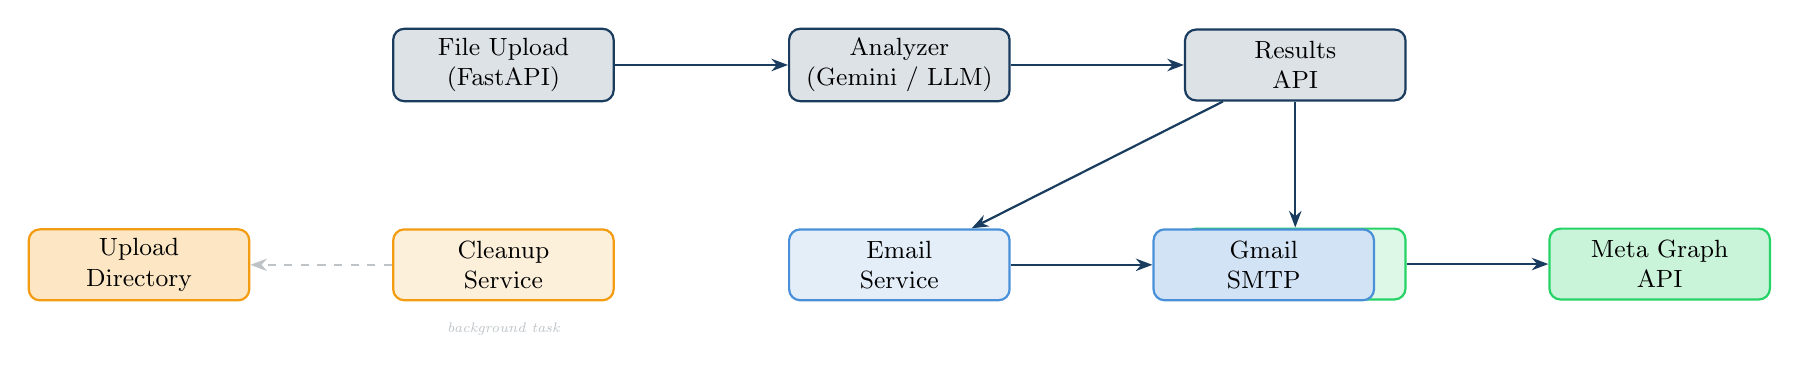
\begin{tikzpicture}[
    node distance = 1.4cm and 2cm,
    every node/.style = {font=\small},
    box/.style = {rectangle, rounded corners=4pt, minimum width=2.8cm,
                  minimum height=0.9cm, draw, thick, align=center},
    arrow/.style = {-{Stealth[length=6pt]}, thick, color=primary},
    dasharrow/.style = {-{Stealth[length=6pt]}, dashed, thick, color=midgray}
  ]
    % Core
    \node[box, fill=primary!15, draw=primary] (upload) {File Upload\\(FastAPI)};
    \node[box, fill=primary!15, draw=primary, right=2.2cm of upload] (analyzer) {Analyzer\\(Gemini / LLM)};
    \node[box, fill=primary!15, draw=primary, right=2.2cm of analyzer] (results) {Results\\API};

    % Services
    \node[box, fill=whatsappgreen!15, draw=whatsappgreen, below=1.6cm of results] (wa) {WhatsApp\\Service};
    \node[box, fill=emailblue!15, draw=emailblue, below=1.6cm of analyzer] (email) {Email\\Service};
    \node[box, fill=warning!15, draw=warning, below=1.6cm of upload] (cleanup) {Cleanup\\Service};

    % External
    \node[box, fill=whatsappgreen!25, draw=whatsappgreen, right=1.8cm of wa] (meta) {Meta Graph\\API};
    \node[box, fill=emailblue!25, draw=emailblue, right=1.8cm of email] (smtp) {Gmail\\SMTP};
    \node[box, fill=warning!25, draw=warning, left=1.8cm of cleanup] (disk) {Upload\\Directory};

    % Arrows
    \draw[arrow] (upload) -- (analyzer);
    \draw[arrow] (analyzer) -- (results);
    \draw[arrow] (results) -- (wa);
    \draw[arrow] (results) -- (email);
    \draw[arrow] (wa) -- (meta);
    \draw[arrow] (email) -- (smtp);
    \draw[dasharrow] (cleanup) -- (disk);

    % Background task label
    \node[font=\tiny\itshape, color=midgray, below=0.15cm of cleanup] {background task};

  \end{tikzpicture}
  \caption{High-level integration of messaging services within TahalilAI}
  \label{fig:architecture}
\end{figure}

% ============================================================
\section{WhatsApp Messaging Service}
% ============================================================

\subsection{Overview}

The WhatsApp service, implemented in \file{backend/src/tahalilai/services/whatsapp.py}
(223 lines), integrates with Meta's \textbf{WhatsApp Cloud API v19.0} to send
patient-facing notifications without any third-party SDK.
The service uses only the Python standard library (\texttt{urllib.request}),
eliminating external dependencies.

\subsection{Public Interface}

The module exposes two public functions that share a common return contract:

\begin{infobox}[title={Return Contract}]
  Success: \quad \texttt{\{"status": "sent", "message\_id": "wamid.xxx"\}} \\
  Failure: \quad \texttt{\{"status": "error", "message": "<human-readable reason>"\}}
\end{infobox}

\subsubsection{\func{send\_whatsapp\_message(to\_phone, message\_text)}}

Sends a plain-text message to a WhatsApp recipient.

\begin{itemize}[leftmargin=*, itemsep=3pt]
  \item \textbf{Input}: E.164-formatted phone number and message text.
  \item \textbf{Truncation}: Messages exceeding 4,096 characters are automatically
        truncated with a trailing ellipsis by the internal \func{\_truncate\_message()}
        helper, respecting the WhatsApp platform limit.
  \item \textbf{Payload}: Serialised as \texttt{application/json} to the
        \texttt{/\{version\}/\{phone\_id\}/messages} endpoint.
  \item \textbf{Timeout}: 30-second network timeout prevents hanging connections.
\end{itemize}

\subsubsection{\func{send\_whatsapp\_document(to\_phone, document\_url, filename, caption)}}

Sends a PDF document via a publicly accessible HTTPS URL.

\begin{itemize}[leftmargin=*, itemsep=3pt]
  \item The \texttt{document\_url} must be a publicly reachable HTTPS link;
        Meta servers will fetch the file independently.
  \item \texttt{filename} defaults to \texttt{"report.pdf"}.
  \item Caption text is capped at 1,024 characters.
\end{itemize}

\subsection{Internal Architecture}

\begin{figure}[H]
  \centering
  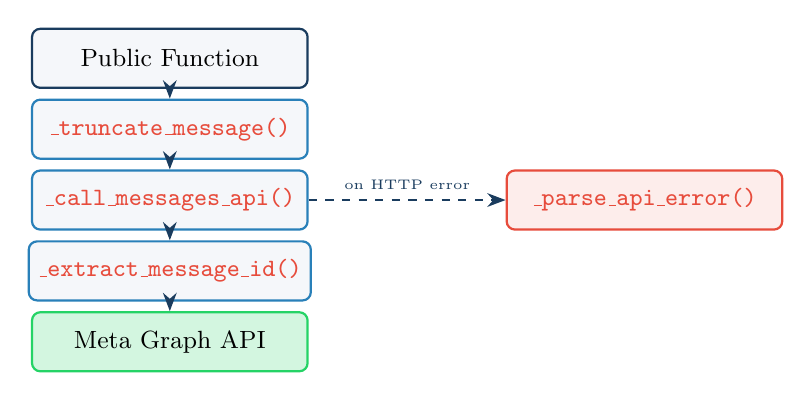
\begin{tikzpicture}[
    node distance=0.9cm and 2cm,
    box/.style={rectangle, rounded corners=3pt, minimum width=3.5cm,
                minimum height=0.75cm, draw, thick, align=center, font=\small},
    arrow/.style={-{Stealth}, thick, color=primary}
  ]
    \node[box, fill=lightgray, draw=primary]   (pub)   {Public Function};
    \node[box, fill=lightgray, draw=accent, below of=pub] (trunc)  {\func{\_truncate\_message()}};
    \node[box, fill=lightgray, draw=accent, below of=trunc] (call)  {\func{\_call\_messages\_api()}};
    \node[box, fill=lightgray, draw=accent, below of=call] (ext)   {\func{\_extract\_message\_id()}};
    \node[box, fill=whatsappgreen!20, draw=whatsappgreen, below of=ext] (meta)  {Meta Graph API};

    \draw[arrow] (pub) -- (trunc);
    \draw[arrow] (trunc) -- (call);
    \draw[arrow] (call) -- (ext);
    \draw[arrow] (ext) -- (meta);

    \node[box, fill=danger!10, draw=danger, right=2.5cm of call] (err) {\func{\_parse\_api\_error()}};
    \draw[arrow, dashed] (call) -- node[above, font=\tiny]{on HTTP error} (err);
  \end{tikzpicture}
  \caption{WhatsApp service internal call chain}
  \label{fig:wa_chain}
\end{figure}

\begin{description}[leftmargin=2em, font=\normalfont\itshape]
  \item[\func{\_call\_messages\_api(settings, payload)}]
    Encodes the payload as UTF-8 JSON, attaches the Bearer token header,
    opens a connection via \texttt{urllib.request.urlopen()}, and returns
    the parsed response body.
  \item[\func{\_extract\_message\_id(body)}]
    Safely navigates \texttt{body["messages"][0]["id"]}; returns
    \texttt{"unknown"} on any \texttt{KeyError} or \texttt{IndexError}.
  \item[\func{\_parse\_api\_error(raw)}]
    Decodes Meta's JSON error envelope to extract
    \texttt{error.message}; falls back to the raw bytes string when
    the response is not valid JSON.
\end{description}

\subsection{Error Handling Strategy}

\begin{longtable}{p{3.5cm} p{5cm} p{5cm}}
  \toprule
  \textbf{Error Class} & \textbf{Trigger} & \textbf{Returned Value} \\
  \midrule
  Credential guard    & Empty token or phone ID   & \texttt{\{"status":"error","message":"..."\}} \\[4pt]
  \texttt{HTTPError}  & 4xx / 5xx from Meta API   & Parsed API error message \\[4pt]
  \texttt{URLError}   & DNS failure, timeout      & System error message \\[4pt]
  Generic \texttt{Exception} & Unexpected failure & Exception string \\
  \bottomrule
  \caption{WhatsApp service error handling matrix}
  \label{tab:wa_errors}
\end{longtable}

\subsection{Configuration}

\begin{longtable}{p{5cm} p{3cm} p{5.5cm}}
  \toprule
  \textbf{Environment Variable} & \textbf{Required} & \textbf{Description} \\
  \midrule
  \envvar{WHATSAPP\_ACCESS\_TOKEN}     & \badge{danger}{Yes} & Meta OAuth2 Bearer token \\[3pt]
  \envvar{WHATSAPP\_PHONE\_NUMBER\_ID} & \badge{danger}{Yes} & Business phone number ID \\[3pt]
  \envvar{WHATSAPP\_API\_VERSION}      & \badge{success}{No} (v19.0) & Graph API version string \\
  \bottomrule
  \caption{WhatsApp service environment variables}
  \label{tab:wa_config}
\end{longtable}

% ============================================================
\section{Email Delivery Service}
% ============================================================

\subsection{Overview}

The email service, implemented in
\file{backend/src/tahalilai/services/email\_sender.py} (197 lines), delivers
medical analysis reports via Gmail's SMTP server over a TLS-encrypted connection
(port 465). It supports multi-language body text (UTF-8) and optional binary
PDF attachments, encoded in Base64 for MIME transport.

\subsection{Public Interface}

\subsubsection{\func{send\_report\_email(recipient\_email, subject, body\_text, pdf\_path)}}

\begin{itemize}[leftmargin=*, itemsep=3pt]
  \item Builds a \texttt{MIMEMultipart} email envelope via the internal
        \func{\_build\_message()} helper.
  \item Optionally attaches a PDF file using \func{\_make\_pdf\_attachment()}.
  \item Connects to Gmail's SMTP server via \func{\_send\_via\_smtp()}.
  \item Returns \texttt{\{"status": "sent"\}} on success, or an error dict.
\end{itemize}

\begin{infobox}[title={MIME Structure}]
  \textbf{With PDF:}\\
  \texttt{MIMEMultipart} \quad\texttt{├── MIMEText} (UTF-8 body)\\
  \hspace*{5.25cm}\texttt{└── MIMEBase} (base64 PDF attachment)\\[6pt]
  \textbf{Without PDF:}\\
  \texttt{MIMEMultipart} \quad\texttt{└── MIMEText} (UTF-8 body)
\end{infobox}

\subsection{Internal Architecture}

\begin{description}[leftmargin=2em, font=\normalfont\itshape]
  \item[\func{\_build\_message(sender, recipient, subject, body\_text, pdf\_path)}]
    Constructs and returns the MIME envelope. Sets \texttt{From}, \texttt{To},
    and \texttt{Subject} headers. Calls \func{\_make\_pdf\_attachment()} when
    a valid \texttt{pdf\_path} is provided.
  \item[\func{\_make\_pdf\_attachment(pdf\_path)}]
    Reads the PDF file in binary mode, base64-encodes the bytes, and attaches
    the \texttt{Content-Disposition: attachment; filename=...} header.
  \item[\func{\_send\_via\_smtp(host, port, sender, password, recipient, message)}]
    Opens an \texttt{smtplib.SMTP\_SSL} context manager on port 465, authenticates
    with the app password, and calls \texttt{sendmail()}.
\end{description}

\subsection{Error Handling Strategy}

\begin{longtable}{p{4cm} p{4.5cm} p{5cm}}
  \toprule
  \textbf{Error Class} & \textbf{Trigger} & \textbf{Returned Value} \\
  \midrule
  Credential guard        & Empty email or app password & Immediate error dict \\[4pt]
  PDF file guard          & Non-existent file path      & Error before SMTP connection \\[4pt]
  \texttt{SMTPAuth\-Error}& Wrong credentials           & User-friendly message \\[4pt]
  Generic \texttt{Exception} & Connection refused, etc. & Exception string \\
  \bottomrule
  \caption{Email service error handling matrix}
  \label{tab:email_errors}
\end{longtable}

\subsection{Configuration}

\begin{longtable}{p{4.5cm} p{3.5cm} p{5.5cm}}
  \toprule
  \textbf{Environment Variable} & \textbf{Default} & \textbf{Description} \\
  \midrule
  \envvar{SMTP\_SENDER\_EMAIL} & \badge{danger}{Required} & Gmail sender address \\[3pt]
  \envvar{SMTP\_APP\_PASSWORD} & \badge{danger}{Required} & 16-character Gmail App Password \\[3pt]
  \envvar{SMTP\_HOST}          & smtp.gmail.com & SMTP server hostname \\[3pt]
  \envvar{SMTP\_PORT}          & 465 & SMTP port (TLS) \\
  \bottomrule
  \caption{Email service environment variables}
  \label{tab:email_config}
\end{longtable}

\begin{warningbox}[title={Security Note}]
  Gmail requires a dedicated \textbf{App Password} (generated at
  \url{https://myaccount.google.com/apppasswords}) rather than the account
  password. The \envvar{SMTP\_APP\_PASSWORD} variable must never be committed
  to version control. The project \file{.gitignore} is configured to exclude
  \file{.env} files.
\end{warningbox}

% ============================================================
\section{Automated Upload Cleanup Service}
% ============================================================

\subsection{Overview}

The cleanup service, implemented in
\file{backend/src/tahalilai/services/cleanup.py} (119 lines), addresses a
practical operational concern: uploaded medical files (images, PDFs) accumulate
on disk after analysis. The service provides:

\begin{itemize}[leftmargin=*, itemsep=3pt]
  \item A \textbf{synchronous} function for on-demand deletion of stale files.
  \item An \textbf{asynchronous loop} that runs as a FastAPI background task,
        periodically invoking the deletion function.
\end{itemize}

\subsection{Public Interface}

\subsubsection{\func{delete\_old\_uploads(uploads\_dir, max\_age\_hours)} \textnormal{(synchronous)}}

\begin{itemize}[leftmargin=*, itemsep=3pt]
  \item Scans \texttt{uploads\_dir} for files older than \texttt{max\_age\_hours}.
  \item Computes staleness as: \texttt{time.time() - file.stat().st\_mtime > max\_age\_hours * 3600}.
  \item Skips files in the \texttt{\_PROTECTED} frozenset (\texttt{.gitkeep})
        and all subdirectories.
  \item Tolerates individual \texttt{OSError} exceptions (e.g., locked files)
        and continues the sweep.
  \item Returns the count of successfully deleted files.
\end{itemize}

\subsubsection{\func{run\_cleanup\_loop(uploads\_dir, max\_age\_hours, interval\_seconds)} \textnormal{(async)}}

\begin{itemize}[leftmargin=*, itemsep=3pt]
  \item Runs indefinitely inside an \texttt{asyncio} task.
  \item \textbf{Sleeps first}, then deletes — ensuring newly uploaded files
        survive at least one full \texttt{interval\_seconds} window.
  \item A top-level \texttt{except Exception} block prevents the task from
        dying on unexpected errors.
  \item Cancelled gracefully via \texttt{asyncio.CancelledError} on server
        shutdown (FastAPI \texttt{lifespan} context).
\end{itemize}

\begin{figure}[H]
  \centering
  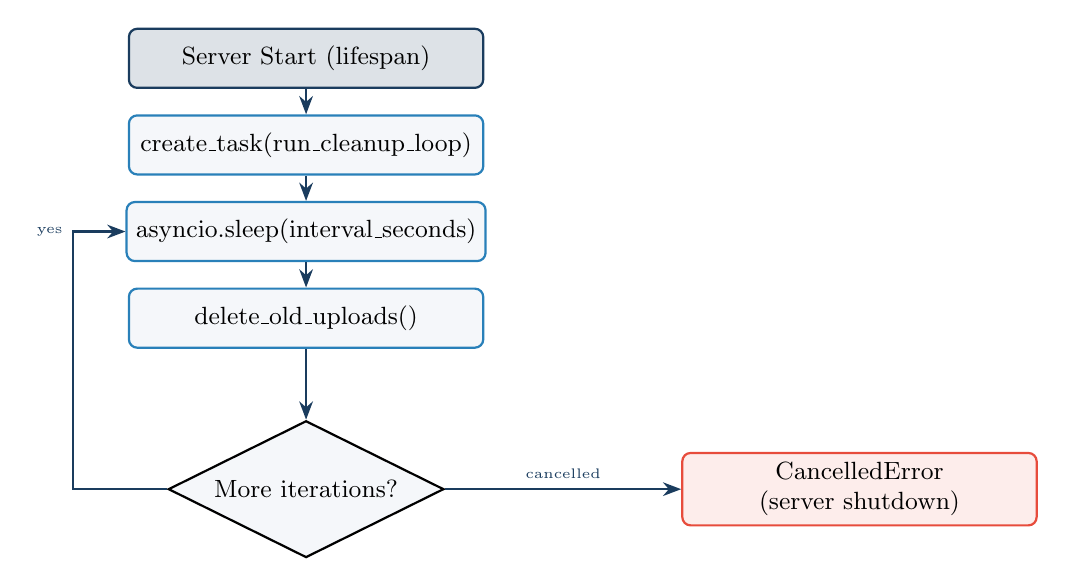
\begin{tikzpicture}[
    node distance=1.1cm,
    box/.style={rectangle, rounded corners=3pt, minimum width=4.5cm,
                minimum height=0.75cm, draw, thick, align=center, font=\small},
    arrow/.style={-{Stealth}, thick, color=primary},
    decision/.style={diamond, draw, thick, aspect=2, font=\small,
                     fill=lightgray, minimum width=3.5cm}
  ]
    \node[box, fill=primary!15, draw=primary] (start)  {Server Start (lifespan)};
    \node[box, fill=lightgray, draw=accent, below of=start] (task)   {create\_task(run\_cleanup\_loop)};
    \node[box, fill=lightgray, draw=accent, below of=task] (sleep)  {asyncio.sleep(interval\_seconds)};
    \node[box, fill=lightgray, draw=accent, below of=sleep] (scan)   {delete\_old\_uploads()};
    \node[decision, below=0.9cm of scan] (decide) {More iterations?};
    \node[box, fill=danger!10, draw=danger, right=3cm of decide] (cancel) {CancelledError\\(server shutdown)};

    \draw[arrow] (start) -- (task);
    \draw[arrow] (task) -- (sleep);
    \draw[arrow] (sleep) -- (scan);
    \draw[arrow] (scan) -- (decide);
    \draw[arrow] (decide.west) -- ++(-1.2,0) |- (sleep.west)
      node[midway, left, font=\tiny]{yes};
    \draw[arrow] (decide) -- (cancel) node[midway, above, font=\tiny]{cancelled};
  \end{tikzpicture}
  \caption{Cleanup service asynchronous loop lifecycle}
  \label{fig:cleanup_loop}
\end{figure}

% ============================================================
\section{Test Suite}
% ============================================================

\subsection{Testing Philosophy}

The test suite is built on \textbf{pytest} with \texttt{unittest.mock}
and follows three principles:

\begin{enumerate}[leftmargin=*, itemsep=3pt]
  \item \textbf{External isolation}: All network calls (Meta API, Gmail SMTP)
        and filesystem mutations are mocked; tests run without any real
        credentials or internet access.
  \item \textbf{Error parity}: Every happy-path function has at least two
        corresponding error-path tests.
  \item \textbf{Behaviour, not implementation}: Tests assert on return values
        and state changes rather than verifying internal call counts.
\end{enumerate}

\subsection{Test Module: WhatsApp Service}
\label{sec:test_wa}

\textbf{File}: \file{backend/tests/unit/test\_whatsapp.py} \quad (191 lines, 14 tests)

\begin{longtable}{p{5.5cm} p{2cm} p{5.5cm}}
  \toprule
  \textbf{Test Case} & \textbf{Class} & \textbf{Assertion} \\
  \midrule
  \texttt{test\_short\_message\_unchanged}        & Truncate & Short text passes unchanged \\
  \texttt{test\_exact\_limit\_unchanged}          & Truncate & 4,096 chars not trimmed \\
  \texttt{test\_long\_message\_truncated}         & Truncate & >4,096 becomes exactly 4,096 with ellipsis \\
  \texttt{test\_valid\_response}                  & ExtractId & Parses \texttt{messages[0].id} \\
  \texttt{test\_missing\_messages\_key}           & ExtractId & Returns \texttt{"unknown"} \\
  \texttt{test\_empty\_messages\_list}            & ExtractId & Returns \texttt{"unknown"} \\
  \texttt{test\_valid\_error\_json}               & ParseErr  & Extracts \texttt{error.message} \\
  \texttt{test\_invalid\_json\_returns\_raw}      & ParseErr  & Returns raw string \\
  \texttt{test\_missing\_credentials\_returns\_error} & SendMsg & Immediate error dict \\
  \texttt{test\_successful\_send}                 & SendMsg & Returns \texttt{"sent"} + message\_id \\
  \texttt{test\_api\_http\_error}                 & SendMsg & 401 caught and returned \\
  \texttt{test\_network\_error}                   & SendMsg & ConnectionError caught \\
  \texttt{test\_missing\_credentials} (doc)       & SendDoc & Immediate error dict \\
  \texttt{test\_successful\_document\_send}       & SendDoc & Document sent with caption \\
  \bottomrule
  \caption{WhatsApp test cases}
\end{longtable}

\textbf{Mock Strategy}:

\begin{lstlisting}[language=Python, caption={WhatsApp mock helpers}]
def _mock_settings():
    s = MagicMock()
    s.whatsapp_access_token = "test-token"
    s.whatsapp_phone_number_id = "12345"
    s.whatsapp_api_version = "v19.0"
    return s

def _mock_urlopen_response(body: dict):
    mock_resp = MagicMock()
    mock_resp.read.return_value = json.dumps(body).encode()
    mock_resp.__enter__ = MagicMock(return_value=mock_resp)
    mock_resp.__exit__ = MagicMock(return_value=False)
    return mock_resp
\end{lstlisting}

\subsection{Test Module: Email Service}
\label{sec:test_email}

\textbf{File}: \file{backend/tests/unit/test\_email\_sender.py} \quad (174 lines, 11 tests)

\begin{longtable}{p{5.5cm} p{2.5cm} p{5cm}}
  \toprule
  \textbf{Test Case} & \textbf{Class} & \textbf{Assertion} \\
  \midrule
  \texttt{test\_missing\_credentials}             & SendEmail & Immediate error dict \\
  \texttt{test\_pdf\_not\_found}                  & SendEmail & Error before SMTP connection \\
  \texttt{test\_successful\_no\_pdf}              & SendEmail & Returns \texttt{"sent"} \\
  \texttt{test\_successful\_with\_pdf}            & SendEmail & Returns \texttt{"sent"} with attachment \\
  \texttt{test\_authentication\_error}            & SendEmail & \texttt{SMTPAuthenticationError} → clear message \\
  \texttt{test\_generic\_error}                   & SendEmail & \texttt{ConnectionRefusedError} caught \\
  \texttt{test\_headers\_are\_correct}            & BuildMsg  & From/To/Subject headers set \\
  \texttt{test\_without\_attachment\_one\_part}   & BuildMsg  & Single MIME part \\
  \texttt{test\_with\_attachment\_two\_parts}     & BuildMsg  & Two MIME parts \\
  \texttt{test\_correct\_filename}                & PDFAttach & Filename in Content-Disposition \\
  \texttt{test\_is\_base64\_encoded}              & PDFAttach & Transfer-Encoding: base64 \\
  \bottomrule
  \caption{Email service test cases}
\end{longtable}

\subsection{Test Module: Cleanup Service}
\label{sec:test_cleanup}

\textbf{File}: \file{backend/tests/unit/test\_cleanup.py} \quad (200 lines, 14 tests)

\begin{longtable}{p{6cm} p{7.5cm}}
  \toprule
  \textbf{Test Case} & \textbf{What It Verifies} \\
  \midrule
  \texttt{test\_returns\_zero\_on\_missing\_dir}  & Non-existent dir → returns 0 \\
  \texttt{test\_deletes\_old\_file}               & File older than threshold is removed \\
  \texttt{test\_keeps\_recent\_file}              & Recent file is preserved \\
  \texttt{test\_deletes\_only\_stale\_files}      & Mixed-age dir: only stale deleted \\
  \texttt{test\_skips\_gitkeep}                   & \texttt{.gitkeep} never deleted \\
  \texttt{test\_skips\_all\_protected\_names}     & All \texttt{\_PROTECTED} entries skipped \\
  \texttt{test\_skips\_subdirectories}            & Directories are never removed \\
  \texttt{test\_tolerates\_oserror}               & Locked file skipped, sweep continues \\
  \texttt{test\_multiple\_file\_types}            & PNG, PDF, MP3 all eligible \\
  \texttt{test\_zero\_max\_age}                   & max\_age\_hours=0 deletes all (except protected) \\
  \texttt{test\_returns\_correct\_count}          & Return value equals files deleted \\
  \texttt{test\_loop\_calls\_delete}              & Loop invokes delete after sleep \\
  \texttt{test\_loop\_logs\_deleted\_count}       & Loop prints summary output \\
  \texttt{test\_loop\_survives\_exception}        & Loop catches exceptions; task does not die \\
  \bottomrule
  \caption{Cleanup service test cases}
\end{longtable}

\textbf{File Age Simulation}:
The \func{\_make\_file()} fixture helper creates a file and back-dates its
modification time using \texttt{os.utime()}, enabling repeatable time-based
tests without sleeping:

\begin{lstlisting}[language=Python, caption={File age back-dating helper}]
def _make_file(tmp_path: Path, name: str, age_hours: float) -> Path:
    p = tmp_path / name
    p.write_text("data")
    past = time.time() - age_hours * 3600
    os.utime(p, (past, past))
    return p
\end{lstlisting}

\subsection{Test Module: Database Models}
\label{sec:test_models}

\textbf{File}: \file{backend/tests/unit/test\_models.py} \quad (243 lines, 17 tests)

The models test module verifies the SQLAlchemy \texttt{Doctor} ORM model using
an in-memory SQLite database to avoid any persistent state between test runs.

\begin{longtable}{p{3.5cm} p{9.5cm}}
  \toprule
  \textbf{Test Class} & \textbf{Coverage} \\
  \midrule
  \texttt{TestDoctorSchema} (3)
    & Table name, table creation, column existence (id, name, city, specialities,
      lat/lng, ratings), composite index \texttt{ix\_doctors\_city\_speciality} \\[4pt]
  \texttt{TestDoctorCRUD} (8)
    & Create/Read/Update/Delete, default values (empty strings for title/phone/address,
      \texttt{None} for coordinates/ratings), nullable fields,
      geocoding and rating field storage \\[4pt]
  \texttt{TestDoctorQueries} (6)
    & Filter by city (\texttt{ilike}), filter by speciality (\texttt{ilike}),
      combined filters, name search, and \texttt{GROUP BY} city counts \\
  \bottomrule
  \caption{Database model test classes}
\end{longtable}

\subsection{Test Module: Doctor Recommender}
\label{sec:test_recommender}

\textbf{File}: \file{backend/tests/unit/test\_recommender.py} \quad (254 lines, 18 tests)

\begin{longtable}{p{4cm} p{9cm}}
  \toprule
  \textbf{Test Class} & \textbf{Coverage} \\
  \midrule
  \texttt{TestCanonical\-Specialities} (4)
    & List non-empty, contains \textit{Médecin généraliste} and \textit{Cardiologue},
      no duplicates \\[4pt]
  \texttt{TestExtract\-Recommended} (7)
    & Default when Gemini unavailable or API key absent; parses valid JSON response;
      strips markdown \texttt{```json} fence; handles API exceptions and invalid JSON;
      truncates long analysis (>3,000 chars) in prompt \\[4pt]
  \texttt{TestFindRecommended\-Doctors} (8)
    & Finds by speciality; city prioritisation; fills from other cities when needed;
      handles multiple specialities; no duplicate doctors; empty speciality list;
      unknown speciality; respects \texttt{limit\_per\_speciality}; verifies
      result schema (id, name, speciality, phone, city, \ldots) \\
  \bottomrule
  \caption{Recommender service test classes}
\end{longtable}

\subsection{Test Coverage Summary}

\begin{figure}[H]
  \centering
  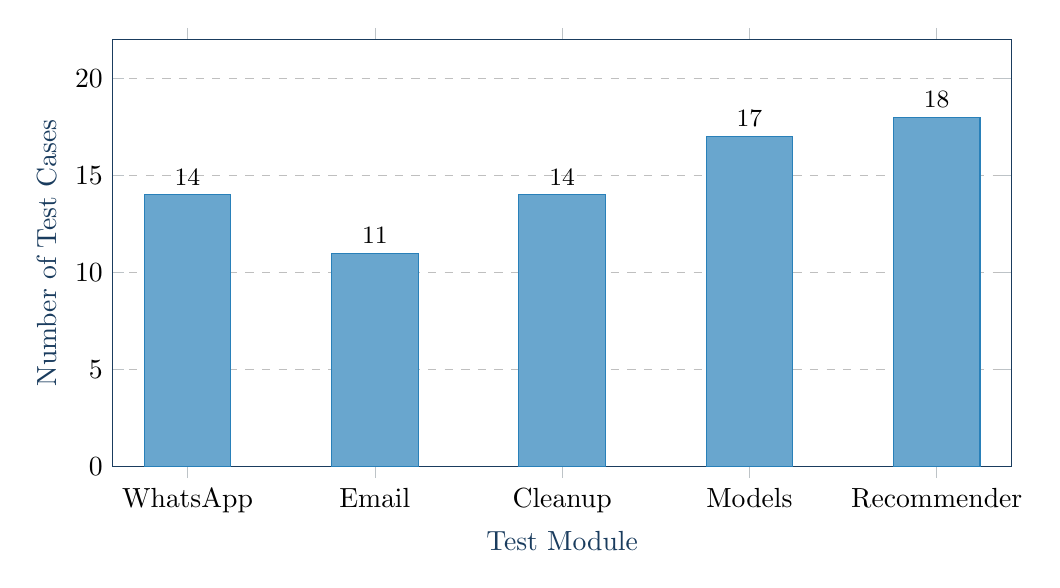
\begin{tikzpicture}
    \begin{axis}[
      ybar,
      bar width=1.1cm,
      width=13cm, height=7cm,
      xlabel={Test Module},
      ylabel={Number of Test Cases},
      symbolic x coords={WhatsApp, Email, Cleanup, Models, Recommender},
      xtick=data,
      ymin=0, ymax=22,
      ymajorgrids=true,
      grid style=dashed,
      nodes near coords,
      nodes near coords align={above},
      every node near coord/.style={font=\small\bfseries},
      axis line style={color=primary},
      tick style={color=midgray},
      label style={color=primary},
    ]
      \addplot[fill=accent!70, draw=accent] coordinates {
        (WhatsApp, 14)
        (Email, 11)
        (Cleanup, 14)
        (Models, 17)
        (Recommender, 18)
      };
    \end{axis}
  \end{tikzpicture}
  \caption{Distribution of unit test cases across modules (total: 74 tests)}
  \label{fig:test_distribution}
\end{figure}

% ============================================================
\section{Design Decisions}
% ============================================================

\subsection{No External Dependency Policy}

Both the WhatsApp service (\texttt{urllib.request}) and email service
(\texttt{smtplib}) deliberately avoid external HTTP client libraries
(\texttt{requests}, \texttt{httpx}, \texttt{aiohttp}).
This decision reduces the dependency surface area, simplifies deployment,
and avoids licence concerns. The trade-off — marginally more verbose code —
is accepted for the reliability benefit.

\subsection{Never-Raise Return Contract}

All public service functions return \texttt{dict[str, str]} on both success
and failure rather than raising exceptions. This contract:

\begin{itemize}[leftmargin=*]
  \item Allows call sites to handle messaging results as data rather
        than control flow.
  \item Simplifies integration with FastAPI background tasks where
        unhandled exceptions would only be silently swallowed.
  \item Makes errors observable without requiring \texttt{try/except}
        at each call site.
\end{itemize}

\subsection{Guard-Clause Pattern}

Each service validates preconditions (credentials, file existence) as the
very first action, before opening any network connection or reading any file.
This fail-fast approach avoids unnecessary resource usage and produces
actionable error messages.

\subsection{Asynchronous Cleanup Design}

The cleanup loop uses \texttt{asyncio.sleep} rather than a blocking
\texttt{time.sleep} so it does not occupy a thread from Python's thread pool.
By sleeping \textit{before} the first deletion, the loop also protects files
uploaded just before the interval boundary.

% ============================================================
\section{Configuration \& Deployment}
% ============================================================

\subsection{Complete Environment Variables Reference}

\begin{longtable}{p{5.5cm} p{3cm} p{5cm}}
  \toprule
  \textbf{Variable} & \textbf{Required} & \textbf{Purpose} \\
  \midrule
  \envvar{SMTP\_SENDER\_EMAIL}          & \badge{danger}{Yes} & Gmail sender address \\
  \envvar{SMTP\_APP\_PASSWORD}          & \badge{danger}{Yes} & Gmail App Password (16 chars) \\
  \envvar{SMTP\_HOST}                   & No (smtp.gmail.com) & SMTP server \\
  \envvar{SMTP\_PORT}                   & No (465) & SMTP TLS port \\
  \envvar{WHATSAPP\_ACCESS\_TOKEN}      & \badge{danger}{Yes} & Meta Bearer token \\
  \envvar{WHATSAPP\_PHONE\_NUMBER\_ID}  & \badge{danger}{Yes} & Meta business phone ID \\
  \envvar{WHATSAPP\_API\_VERSION}       & No (v19.0) & Graph API version \\
  \bottomrule
  \caption{All environment variables introduced by the messaging services}
\end{longtable}

\subsection{Running the Test Suite}

\begin{lstlisting}[language=bash, caption={Executing unit tests}, style=pythonstyle]
# From the backend directory
cd backend

# Run all unit tests
pytest tests/unit/ -v

# Run a specific module
pytest tests/unit/test_whatsapp.py -v
pytest tests/unit/test_email_sender.py -v
pytest tests/unit/test_cleanup.py -v
pytest tests/unit/test_models.py -v
pytest tests/unit/test_recommender.py -v

# Generate coverage report
pytest tests/unit/ --cov=tahalilai.services --cov-report=term-missing
\end{lstlisting}

% ============================================================
\section{Summary and Conclusion}
% ============================================================

This report has documented the complete design and implementation of three
production-grade backend services added to the TahalilAI platform:

\begin{enumerate}[leftmargin=*, itemsep=5pt]
  \item \textbf{WhatsApp Service} — A zero-dependency, stdlib-only integration
        with Meta's Cloud API that sends both text notifications and PDF
        document reports to patients, handling all network and credential errors
        gracefully.
  \item \textbf{Email Service} — A MIME-aware SMTP client that delivers medical
        analysis reports with or without PDF attachments over a TLS-secured
        Gmail connection, with specific handling for authentication failures.
  \item \textbf{Upload Cleanup Service} — An asynchronous background worker
        that prevents uncontrolled disk growth by periodically purging stale
        upload files, while protecting version-control placeholders and
        tolerating individual file system errors.
\end{enumerate}

The accompanying \textbf{74-test suite} (across 5 modules) validates all
services, their internal helpers, and their error-handling branches without
requiring any live credentials or network access.

\begin{successbox}[title={Deliverables Completed}]
  \begin{itemize}[leftmargin=*, itemsep=3pt, topsep=0pt]
    \item[\checkmark] \file{services/whatsapp.py} — 223 lines, 2 public functions
    \item[\checkmark] \file{services/email\_sender.py} — 197 lines, 1 public function
    \item[\checkmark] \file{services/cleanup.py} — 119 lines, 2 public functions
    \item[\checkmark] \file{tests/unit/test\_whatsapp.py} — 14 tests
    \item[\checkmark] \file{tests/unit/test\_email\_sender.py} — 11 tests
    \item[\checkmark] \file{tests/unit/test\_cleanup.py} — 14 tests
    \item[\checkmark] \file{tests/unit/test\_models.py} — 17 tests
    \item[\checkmark] \file{tests/unit/test\_recommender.py} — 18 tests
  \end{itemize}
\end{successbox}

\vspace{1cm}
\begin{center}
  \color{midgray}\small
  \textit{TahalilAI Engineering Development Report — Version 1.0 — March 2026}\\
  \textit{Generated for academic review. All implementation details reflect the current codebase.}
\end{center}

\end{document}
